\appendix

% ---- Apéndice con las capturas del Datasheet en Vertical UwU
\newpage
\section*{Apéndice: Curvas de referencia del fabricante (Datasheet 4N25)}
\label{sec:apendice}

En esta sección se adjuntan los gráficos extraídos de la hoja de datos oficial del fabricante (Vishay Semiconductor) utilizados para la normalización y comparación de los parámetros ensayados.

\begin{figure}[H]
    \centering
    % Captura 1 - Curva CTR no saturada (the classic one)
    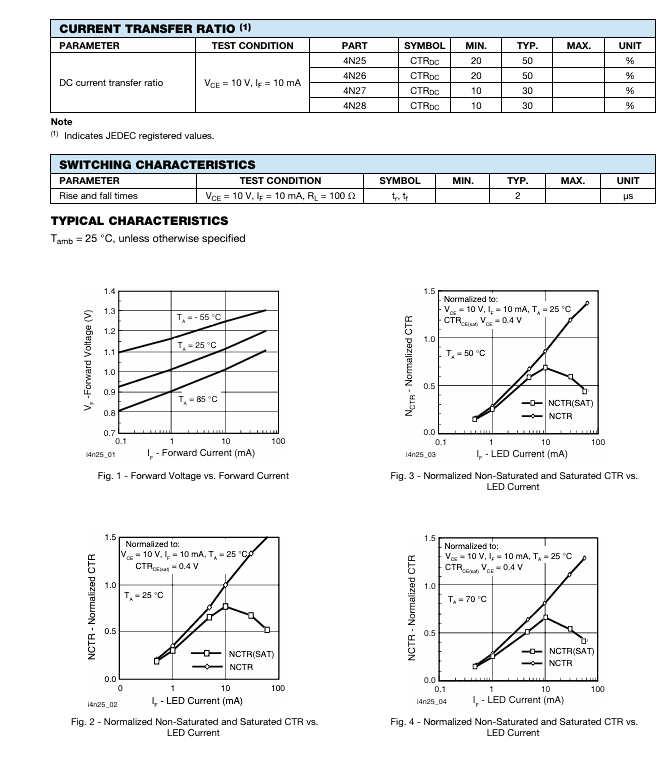
\includegraphics[width=0.75\linewidth]{img/data_1.png}
    \caption{CTR Normalizado vs. $I_F$ en zona activa (Vishay).}
    \label{fig:data_1}
\end{figure}

\begin{figure}[H]
    \centering
    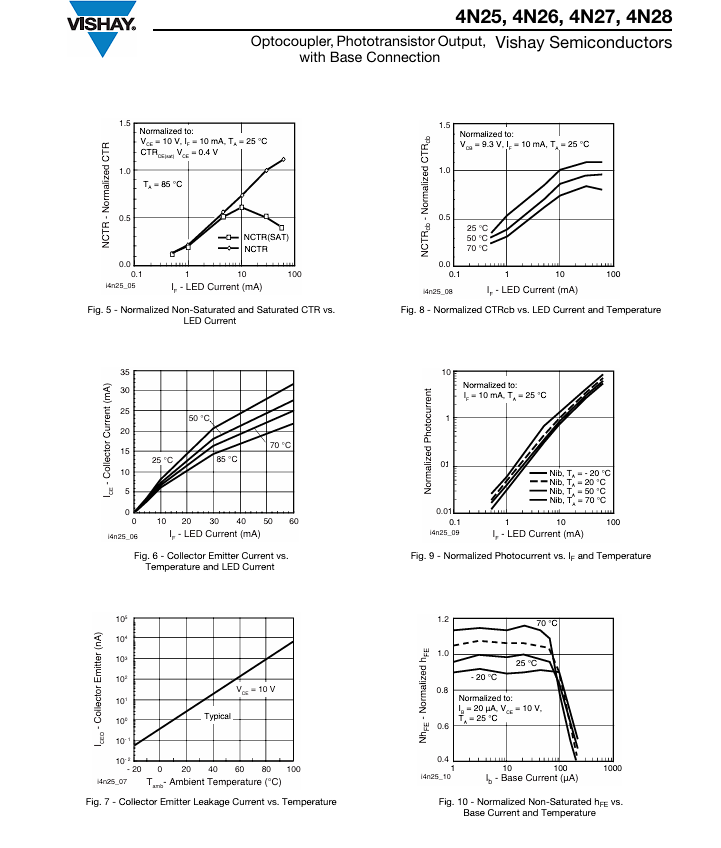
\includegraphics[width=0.75\linewidth]{img/data_2.png}
    \caption{CTR Normalizado en saturación (Vishay).}
    \label{fig:data_2}
\end{figure}

\begin{figure}[H]
    \centering
    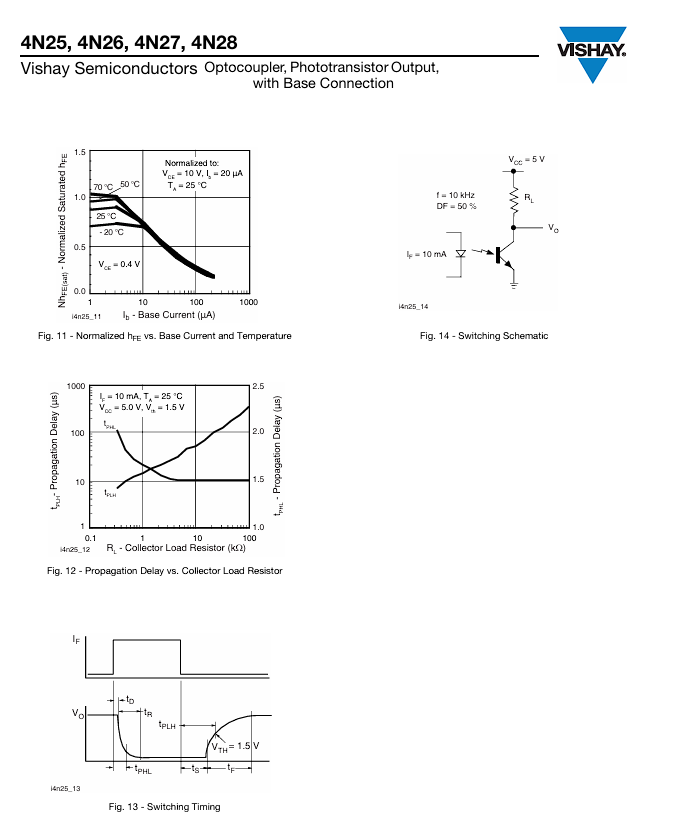
\includegraphics[width=0.75\linewidth]{img/data_3.png}
    \caption{Tiempos de conmutación en función de $R_L$ (Vishay).}
    \label{fig:data_3}
\end{figure}